\section{Simulation model}
\label{sec:mskmodel}

This section gives a description of the model implemented by the
simulator, without references to specific parameter names in the XML
configuration file.
See the next section for example configuration files,
section~\ref{sec:mskxml}
for a primer on XML and the data types used in parameter files,
and
the HTML documentation of the XML Schemas of ContactCenters for more
information on parameter names.

Figure~\ref{fig:ccmodel} gives an overview of the model implemented by
the simulator.  It shows that
calls are partitioned into $K$ \emph{call types} and
are sent to
agents partitioned into $I$ \emph{agent groups}.
Inbound calls arrive in the center from external sources while
outbound calls are produced by predictive dialers which are part of
the call center.
Calls that cannot be served immediately are queued, and abandon
if they cannot get service after a certain patience time.
However, the model is more complex than the figure shows:
the queueing discipline is not always first-in first-out,
routing can consider agents with multiple skills, and
parameters can change during the day.
The next sections will examine these aspects in more details.
%It can simulate multiple periods with different parameters in each
%one.  Inbound and outbound calls are supported as well as skill-based
%routing.

\begin{figure}
\centering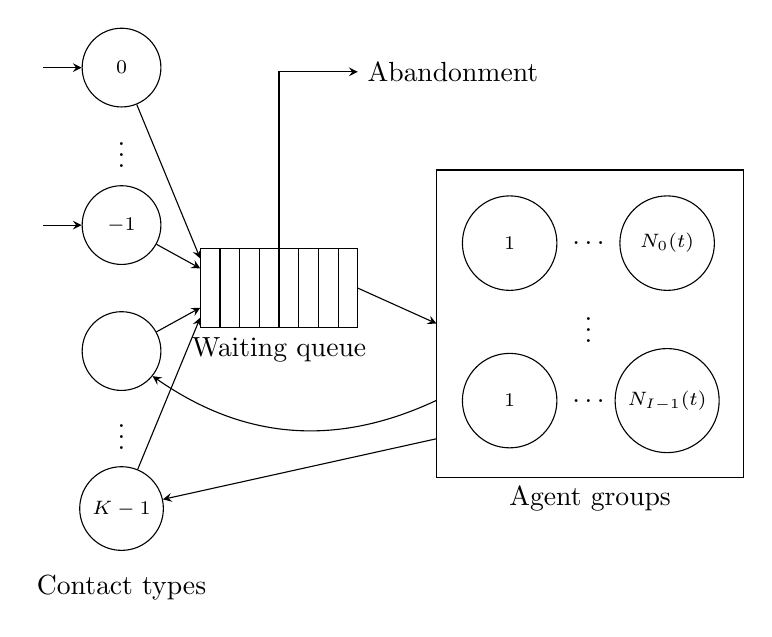
\begin{tikzpicture}[>=stealth]

\node (a1) [shape=circle,draw,minimum size=1.2cm] {{\scriptsize 1}};
\node (ai) [right of=a1] {$\ldots$};
\node (an) [right of=ai,circle,draw,minimum size=1.2cm] {{\scriptsize $N_0(t)$}};
\node (mid1) [below of=a1,shape=coordinate] {};
\node (mid) [below of=ai] {$\vdots$};
\node (midn) [below of=an,shape=coordinate] {};
\node (a21) [shape=circle,draw,below of=mid1,minimum size=1.2cm] {{\scriptsize 1}};
\node (a2i) [below of=mid] {$\ldots$};
\node (a2n) [below of=midn,circle,draw,minimum size=1.2cm] {{\scriptsize $N_{I-1}(t)$}};

\draw (a1.north west) +(-5mm,5mm) coordinate(topleftcorner)
(a2n.south east) +(5mm,-5mm) coordinate(bottomrightcorner);
\draw (topleftcorner) rectangle (bottomrightcorner);
\draw (topleftcorner |- bottomrightcorner) coordinate(bottomleftcorner);
\draw (topleftcorner -| bottomrightcorner) coordinate(toprightcorner);

\draw (topleftcorner) ++(-3,-2) coordinate(qbottomleftcorner)
rectangle ++(2,1) coordinate(qtoprightcorner);
\foreach \x in {0,0.25,...,2}
   \draw (qbottomleftcorner) ++(\x,0)
-- +(0,1);

\draw (qtoprightcorner |- qbottomleftcorner)
coordinate(qbottomrightcorner);
\draw (qtoprightcorner -| qbottomleftcorner)
coordinate(qtopleftcorner);

\path (bottomleftcorner)
 -- node [below] {Agent groups} (bottomrightcorner);
\path (qbottomleftcorner)
-- node [below] {Waiting queue} (qbottomrightcorner);

\draw (qtopleftcorner) ++(-1,2.3) node (k0) [shape=circle,draw,minimum size=1cm] {{\scriptsize $0$}};
%\node (kk) [below of=k0] {$\vdots$};
\draw (qtopleftcorner) ++(-1,0.3)
node (kK) [shape=circle,draw,minimum size=1cm]
{{\scriptsize $\Ki-1$}};
\path (k0) to
node (kk) {$\vdots$}
(kK);
\node (k0l) [left of=k0,shape=coordinate] {};
\draw[->] (k0l) -- (k0);
\node (kKl) [left of=kK,shape=coordinate] {};
\draw[->] (kKl) -- (kK);
\draw (qbottomleftcorner) ++(-1,-0.3)
node (ko0) [shape=circle,draw,minimum size=1cm] {{\scriptsize $\Ki$}};
\draw (qbottomleftcorner) ++(-1,-2.3)
node (koK) [shape=circle,draw,minimum size=1cm] {{\scriptsize $K - 1$}};
\path (ko0) to
node (kok) {$\vdots$}
(koK);
\node [below of=koK] {Contact types};

\path (qtopleftcorner) -- 
coordinate [very near start] (qcenterleft1)
coordinate [near start] (qcenterleft2)
coordinate [near end] (qcenterleft3)
coordinate [very near end] (qcenterleft4) (qbottomleftcorner);
\draw[->] (k0) -- (qcenterleft1);
\draw[->] (kK) -- (qcenterleft2);
\draw[->] (ko0) -- (qcenterleft3);
\draw[->] (koK) -- (qcenterleft4);
\path (topleftcorner) --
coordinate [near end] (centerleft1)
coordinate [very near end] (centerleft2)
(bottomleftcorner);
\draw[->] (centerleft1) to [bend left] (ko0);
\draw[->] (centerleft2) -- (koK);

\path (qtoprightcorner) -- 
coordinate (qcenterright)
(qbottomrightcorner);
\path (topleftcorner) --
coordinate (centerleft)
(bottomleftcorner);
\draw [->] (qcenterright) -- (centerleft);

\draw (topleftcorner) ++(-1,1) node (ab) [above right] {Abandonment};
\path (qtopleftcorner)
--
coordinate(qtopcenter)
(qtoprightcorner);
\draw[->] (qtopcenter) |- (ab);
\end{tikzpicture}


\caption{The Implemented Model of Call Center}
\label{fig:ccmodel}
\end{figure}

\subsection{The simulation horizon divided into periods}
\label{sec:periods}

The simulation horizon can correspond to a day, a week, a month, etc.
As shown on figure~\ref{fig:periods},
it is divided into $P+2$ time
intervals called \emph{periods}.
The call center's opening hours are divided into $P$ \emph{main periods}
with fixed duration $d$.
For example, these periods may correspond to
half hours or hours in
the simulated horizon.
Main period~$p=1,\ldots,P$ corresponds to the
time interval $[t_{p-1}, t_p)$, where $0 \le t_0 < \cdots < t_P$.
During the \emph{preliminary period} $[0, t_0)$, no agent is available
to serve calls but arrivals can start a few minutes before $t_0$ for a
queue to build up.
During the \emph{wrap-up period} $[t_P, T]$, where $T$ is the time at
which the simulation ends and the center is completely empty, no
arrival occurs, but in-progress services are terminated.

\begin{figure}
\centering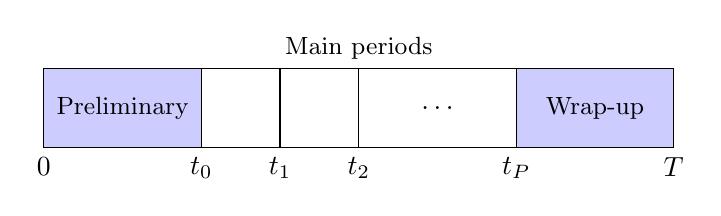
\begin{tikzpicture}[>=stealth]
\draw [fill=blue!20] (0,0) rectangle (2,1);
\draw [fill=blue!20] (6,0) rectangle (8,1);
\draw (0,0) rectangle (8,1);
\foreach \x/\xtext in {0, 2/$t_0$, 3/$t_1$, 4/$t_2$, 6/$t_P$, 8/$T$}
    \draw (\x,1) -- ++(0,-1) node [below] {\xtext};
\node at (1,0.5) {{\small Preliminary}};
\node at (5,0.5) {$\ldots$};
\node at (7,0.5) {{\small Wrap-up}};
\node at (4, 1) [above] {{\small Main periods}};
\end{tikzpicture}


\caption{The simulated horizon}
\label{fig:periods}
\end{figure}

Parameters are usually specified for the main periods only.  During
the preliminary
period, there are no agents to serve calls and if other parameters are
needed, the simulator takes them from the first main
period.  During the wrap-up period, the parameters from the last main
period are used.
The preliminary and wrap-up periods can have a length of 0
in several models.  They are useful to simulate one day starting where
$t_0>0$.  Since the preliminary and wrap-up periods are secondary,
main periods are often denoted as
the periods in the rest of this document.

\subsection{The processing of a call}

The set of $K$ call types is divided into two subsets:
$\Ki\le K$ inbound call types with indices $0, \ldots, \Ki - 1$,
and $\Ko$ outbound call types with indices $\Ki, \ldots, K - 1$.
Each call type can have its own \emph{call source} which produces
only calls of this type, and can be
shut up and down at any time during the simulation.
In addition, call sources producing calls of multiple, randomly-chosen
types, can be defined.
In the latter case, if a call is generated during main period~$p$,
its type is $k$ with a fixed probability
$p_{k,p}$,
independently of other calls.
The way calls are produced depends on whether they are inbound or
outbound, and will be covered in the next subsections.
% The \emph{service time}, i.e., the time spent by a call with an agent,
% can depend on the period~$p$ of arrival,
% the call type~$k$ as
% well as the agent group~$i$ assigned by the router.
% Let $1/\mu_{k, p}$ be the call type-dependent mean service time and
% $1/\mu_{k,
%   i, p}$ be the mean service time depending on call type and agent group.

% A call of type~$k$ entering the system during period~$p$ that cannot
% be served
% immediately balks, i.e., abandons
% without being served or waiting in queue, with probability $\pi_{k,
%   p}$.  If it does not balk,
% before abandoning or being served, it waits for a maximal
% \emph{patience time} with mean $1/\nu_{k,p}$, which can have any
% period-specific probability distribution.

Figure~\ref{fig:callpath} shows the path of a call into
the call center.
On this figure, rectangles represent processing steps for
the call while diamonds represent conditional branching.
The rectangle with thick lines represents the starting point of the
calls in the system.
An ellipse denotes an outcome for a call (blocking, service,
or abandonment).
When a call arrives, a free agent is selected among the $I$ agent groups.
The router (see section~\ref{sec:routergeninfo}) uses
the type of the call to determine
which agents are allowed to serve the call,
and how agents are chosen if several agents are free.
If a free agent is found, the call is sent to that agent, and
the agent is allocated for a certain \emph{service time}.
Conditionally on the call type, agent group and period of arrival of
the call, service times are i.i.d.\ and follow any parametric
probability distribution supported by SSJ.
If no agent is available for a new call, the call is sent to a waiting
queue if that does not exceed the total queue capacity.
With some probability depending on the call type
and the arrival period, independently of other events, the caller
entering queue
\emph{balks}, i.e., it abandons
immediately.  Other calls
having to wait go into a queue where they remain
until agents are free to serve them.
A queued caller can also become impatient, and abandon without
service.
Patience times are i.i.d.\ conditional to call type, and arrival period.
If the queue is full at the time of a call's arrival,
the call is \emph{blocked} instead of entering the queue, i.e., the
caller
receives a busy signal.

\begin{figure}
\centering\begin{tikzpicture}[shape=rectangle,>=stealth]
\node (ap) [draw,line width=2pt] {Enter system};
\node (ifq) [draw,shape=diamond, node distance=5cm, below of=ap] {Queue full?};
\node (ifa) [draw,shape=diamond, node distance=5cm, right of=ap, text width=3cm] {At
  least one free agent?};
\node (balk) [draw,shape=diamond, node distance=5cm, right of=ifq]
{Balking?};
\node (q) [draw, right of=balk, node distance=3cm] {Queue};
\node (ifp) [draw,shape=diamond, node distance=4cm, right of=q, text width=2.5cm]
{Patience time exceeded?};

\node (bl) [draw, shape=ellipse, below of=ap] {Blocking};
\node (sr) [draw, right of=ifa, node distance=6cm, shape=ellipse] {Service};
\node (ab) [draw, below of=sr, shape=ellipse] {Abandonment};

\draw[->] (ap) -- (ifa);
\draw[->] (ifq) edge 
node [left] {Yes}
(bl)
edge 
node [above] {No}
(balk);
\draw[->] (ifa) edge
node [above] {Yes}
(sr)
edge
node [above] {No}
(ifq);
\draw[->] (balk)
edge [bend left]
node [above] {Yes}
(ab)
edge
node [above] {No}
(q);
\draw[->] (q) -- (ifp);
\draw[->,bend angle=85] (ifp)
edge
node [right] {Yes}
(ab)
edge [bend right]
node [right] {No}
(sr);
\end{tikzpicture}


\caption{The path of a call in the call center}
\label{fig:callpath}
\end{figure}

An agent finishing a service can disconnect for a random duration
before it takes new calls.
The probability and duration
of disconnecting may depend on the agent group, and
the time period.
By default, the probability is 0, so no disconnecting occurs.

\subsubsection{Inbound calls}

\emph{Inbound calls} are produced using
some \emph{arrival processes}.  Such a process generates
random inter-arrival times following some possibly
non-stationary distributions, and generates a single call upon each
arrival.  The most common distribution for inter-arrival times is
exponential, which results in a Poisson arrival process.
The simulator supports some variants of the Poisson process with
time-varying or stochastic arrival rates.
See
section~\ref{javadoc:umontreal.iro.lecuyer.contactcenters.app.ArrivalProcessType}
for more details.

\subsubsection{Outbound calls}

\emph{Outbound calls} are produced
using a predictive \emph{dialer}
which makes outbound calls when
certain conditions apply.  There can be one dialer for each outbound call
type as well as dialers producing outbound calls of multiple,
randomly-chosen, types.

When a dialer is started, it tries to perform outbound calls
each time an agent capable of serving calls produced by the
dialer becomes free.
Each time the dialer is triggered, it decides on how many calls to
try, and processes each of these calls independently,
as shown on
figure~\ref{fig:outbound}.
First, dialing succeeds with a reaching
probability depending on the call type and period.
A delay depending on the success of the call, the call type, and the
period of dialing then occurs.
The dialing delay can be used to model the party's phone ringing while
a failed call may represent a busy signal, answering machine, etc.
Successful calls are processed in a similar
way as inbound calls while failed calls simply leave the system after
they are counted.
During the processing of a successful call, the period of arrival
corresponds to the period during which the dialer decided to make a
call, not the period during which the call entered the call center.

The only difference when processing inbound calls and successful
outbound calls is
the service time which includes a \emph{preview time} that
can be used to model the work made by the agent to determine
if the right party is reached.
The same way as service times,
preview times are i.i.d.\ but can depend on the call type, agent
group,
and period of arrival.
After this preview time,
with some probability depending on the call type and period of
arrival, the call is a right party connect, and enters regular service.
The preview and regular service times are generated
independently, and summed up in the case of right party connects. In other words,
the time the agent spends with an outbound
call is the sum of the preview and service times.
On the other hand,
if the call is a wrong party connect, it is counted separately and
excluded from reports concerning served calls.
The service of a wrong party connect only consists of a preview time.

No further special processing is applied to outbound calls
in this model.  However, some parameters can
be adapted to outbound calls.
For example, a called customer often balks (or
abandons very quickly) if no agent is available to serve him.
In fact, any outbound call that needs to wait is called a
\emph{mismatch}, and
is avoided in most call centers.
Consequently, the average patience time of any outbound call should be
small.

\begin{figure}
\centering\begin{tikzpicture}[shape=rectangle,>=stealth]
\node (dialing) [draw, line width=2pt] {Dialing};
\node (rpc) [draw, shape=diamond, node distance=5cm, right of=dialing,
text width=2.5cm]
{Reached call?};
\node (failtime) [draw, node distance=3cm, above of=rpc]
{Fail delay};
\node (fail) [draw, shape=ellipse, right of=failtime, node distance=3cm]
{Failing};
\node (reachtime) [draw, node distance=5cm, below of=dialing]
{Reach delay};
\node (ib) [draw, shape=ellipse, node distance=5cm, right
of=reachtime]
{Enter system};


\draw[->] (dialing) -- (rpc);
\draw[->] (rpc)
edge
node [left] {Yes}
(reachtime)
edge
node [left] {No}
(failtime);
\draw[->] (failtime) -- (fail);
\draw[->] (reachtime) -- (ib);
\end{tikzpicture}


\caption{The path of an outbound call in the call center}
\label{fig:outbound}
\end{figure}

The dialer uses a \emph{dialer's policy} to determine how many calls
to dial each time it is triggered.
%For this, the policy often uses the number of agents in a \emph{test
%  set} of groups that contains all agent groups in the call center.
%The set of agent groups from which the dialer gets the number of free
%agents capable of serving the dialed calls is named the \emph{target
%  set}, and the target set for dialer~$k$ is composed of all agents
%capable of serving calls of any type produced by that dialer.
Let $\Ntf(t)$ be the total number of free agents, or
equivalently the number of free agents in the \emph{test set}, at simulation
time~$t$.  Also let
$\Ndf[k](t)$ be the total number of free agents capable of serving
some calls produced by dialer~$k$, or equivalently the number of free agents in the
\emph{target set} for dialer~$k$, at simulation time~$t$.

A common dialing condition checks that $\Ntf(t)\ge s_{\mathrm{t}, k}(t)$,
and $\Ndf[k](t)\ge s_{\mathrm{d}, k}(t)$, where
$s_{\mathrm{t}, k}(t)$ and
$s_{\mathrm{d}, k}(t)$ are user-defined thresholds. Their values are
constant during periods but can change from periods to periods.
The number of calls to dial at a time is computed from $\Ndf[k](t)$ in
a way depending on the selected \emph{dialing policy}.
See
section~\ref{javadoc:umontreal.iro.lecuyer.contactcenters.app.DialerPolicyType}
for more information.

% When an outbound call of type~$k$ is made during period~$p$,
% a \emph{right party connect} occurs with
% probability
% $\rho_{k, p}$.  When a right party connect occurs, the resulting successful call
% reaches the router for further processing.
% Otherwise, the call is
% a failed call which is counted for statistical collecting only before it
% disappears.  Some period-specific
% random delay, which is set to~0 by default,
% is needed for the dialer to determine if a call
% succeeds or fails.

\begin{comment}
\subsection{The attributes of a call}
\label{sec:callattr}

At the time of its creation, a call gets some attributes: a type index
$k$, a
patience time, and $I$ service times.
All these attributes are random variates generated at the time the
call arrives.
The call type determines the distribution of these
random variables as well as a period-specific probability of balking,
When balking occurs, the patience time is 0 independently of the
specified distribution.
The patience time is used for abandonment while the
service time $i$ is used if the call is served by an agent in group~$i$.
The $I$ service times are equal if service times do not depend on the
selected agent.

Acceptable waiting times $s_{k, \pawt}$, $\sK{k}$,
$\sP{\pawt}$, and $s$ are thresholds
used for estimating quantities such as the service level
in the case of inbound calls.
These thresholds, which are often equal, depend only on the call type,
and the AWT period $\pawt$ of the call, the latter period
index depending on how the simulation is performed.
For a simulation on a finite horizon  (see section~\ref{sec:simoutput}),
$\pawt$ corresponds to the statistical period $\pstat$ of the call,
which usually corresponds to its period of arrival.
For a steady-state simulation,
$\pawt$ corresponds to the period simulated at steady state.
%The threshold used depends on the call type and
%time interval for which the
%performance measure is estimated.
For example, the number of calls of type~$k$ during the whole horizon
served before the threshold is determined using $\sK{k}$ while the
number of calls of type~$k$ and statistical period $\pstat$
is determined using $s_{k, \pawt}$.

Outbound calls have additional attributes: the
result of a test determining if it succeeds (i.e., right party
connect) or fails, and
the random delays between the time the dialing and
the success or failure of the call.
The outbound call type determines the probability of right party
connect for each main period as well as the distribution for reach and
fail times.

After it exits the system, a call gets some additional attributes: a
waiting time (which can be 0 if the call was served immediately), and
a statistical period $\pstat$.  This second period index
also depends on how the simulation is performed, but it usually
also corresponds to the period of arrival of the call.
Table~\ref{tab:callperiods} gives the default value of the AWT and
statistical periods for both supported experiment types.

\begin{table}
\caption{The periods of a call}
\label{tab:callperiods}

\centering
\begin{tabular}{|l|l|l|} \hline
Horizon & $\pawt$ & $\pstat$ \\ \hline
Finite (see section~\ref{sec:expfinite}) & $\pstat$
& Period of arrival \\
Infinite (see section~\ref{sec:expsteadystate}) & $p$ & 0 \\
\hline
\end{tabular}
\end{table}
\end{comment}

\subsection{The agent groups}

Each agent group~$i$ has a fixed number $N_i(t)$  of agents
at any time during the simulated horizon.
%This number can
%change from periods to periods, but is often constant inside
%a period.
In this model, the function $N_i(t)$ is piecewise-constant.
If $N_i(t)$ increases at a given time $t$, the additional
agents are notified to the router which assigns them queued calls, if
possible.
The type of the queued call assigned to a new agent in group~$i$
depends on the routing policy being used.

Often, agents are added in several groups at a given time $t$,
corresponding, e.g., to the beginning of a main period.
In such a case, the router notifies all new agents in group~0 to the
router before notifying agents in groups~1, 2, etc.
The order in which the agents are notified to the router may have a
small impact on which queued calls are assigned to which agent groups,
but this only affects a few calls.

If $N_i(t)$ decreases at a given time $t$, no particular event
happens, except if $N_i(t)$ becomes smaller than
$\Nb[i](t)$.
The behavior of the system when that occurs
depends on how the agent group is modeled, but an agent
always terminates its on-going service before it can leave.

Only a fraction of the available agents is allowed to
serve calls.  If there is no busy agent, the total number of
agents free to serve calls is given by $\epsilon_i N_i(t)$ rounded to
the nearest integer, where $\epsilon_i\in[0, 1]$ is the
\emph{efficiency} of the agent group.  If $\epsilon_i=1$, all agents
are allowed to serve calls.

Agent groups can be modeled two ways by the simulator: with counters
representing the number of agents in each state, or with entities
representing each individual agent.
With the first model, the agent group only retains the number of
agents which are busy, free, and idle but unavailable to serve calls.
When $N_i(t)<\Nb[i](t)$, on-going services
are finished, and the group does not accept any call until
$\Nb[i](t) < N_i(t)$.
However, in the second model, the so-called \emph{detailed} group is
composed of
separate agents with their own states.
In that case, when $N_i(t)<\Nb[i](t)$,
some agents are marked to leave the system, but other busy agents
might finish their services before these marked agents leave.
As a
result, a detailed group can accept new calls even when
$\Nb[i](t)>N_i(t)$.
Which agents are marked is not relevant, because all busy agents are
identical in the model.
Detailed agent groups are more realistic, and allow for computing the
longest idle time of agents, which is needed by some routing
policies. However, using counter-based agent groups can increase
performance compared to detailed groups.

The $N_i(t)$ functions can be specified three ways: with a staffing
vector, with a schedule, or with individual agents.
In the first setting, $N_i(t)$ remains constant during individual
periods.
When specifying a schedule, one gives a set of shifts with arbitrary
starting and ending times, and assigns some agents to each shift.
With the third mode, one assigns each individual agent
any user-defined properties in addition to a shift.

\subsection{The router}
\label{sec:routergeninfo}

A \emph{router} assigns agents to inbound calls and successful
outbound calls (\emph{agent selection} or
\emph{push routing}), and
queued calls to free agents (\emph{call selection} or
\emph{pull routing}), using
a \emph{routing policy} to take its decisions.
The model supports a set of predefined routing policies (see
section~\ref{javadoc:umontreal.iro.lecuyer.contactcenters.app.RouterPolicyType})
that can be parametrized by the user.

The waiting queue
represented on figure~\ref{fig:ccmodel}
is partitioned into several
elementary waiting queues implemented as lists.
The number of waiting queues,
and the way they are used
depends on the routing policy.  Most routing policies assign a
waiting queue to each contact type, and all policies supported by the
simulator use a First In First Out (FIFO) discipline in individual
queues.

Parameters for the routing policy are encoded in one of the three main data
structures: a set of ordered lists,
incidence matrices, or matrices of ranks.  When the first
structure is used, the
\emph{type-to-group map} defines an ordered list of agent groups
$i_{k, 0}, i_{k, 1}, \ldots$ for each call type~$k$.  These lists give the order
in which agent groups are tested during agent selection.
The \emph{group-to-type map} defines an ordered list
of call types $k_{i, 0}, k_{i, 1}, \ldots$ for each agent group~$i$.  These lists
are used during call selection to determine the order in which
call types are tested.
These routing tables are represented by non-rectangular 2D arrays of integers.
In the type-to-group map, there is one row for each call type whereas
in the group-to-type map, there is one row per agent group.
Any negative integer
in these 2D arrays being ignored, they can be used for padding.
For an example of a routing policy using this structure, see
\texttt{QUEUEPRIORITY} in
section~\ref{javadoc:umontreal.iro.lecuyer.contactcenters.app.RouterPolicyType}.

The second possible structure is a pair of incidence matrices.
The \emph{type-to-group incidence matrix}
defines a
boolean function $\iTG(k, i)$ which determines if
calls of type~$k$ can be routed to agents in group~$i$.
The \emph{group-to-type incidence matrix}
defines a similar function
$\iGT(i, k)$ that determines if a call of type~$k$ can be selected
by a free agent in group~$i$.
Often, $\iTG(k, i)=\iGT(i, k)$, i.e., a call of type~$k$ can be sent
to an agent in group~$i$ if and only if a free agent in group~$i$
can select a call of type~$k$.
These matrices are encoded into 2D arrays of booleans.
This structure is not used by any router at this moment.

When the third structure is used,
the \emph{matrices of ranks}, which can also be named the priority matrices,
define functions
$\rTG(k, i)$ and
$\rGT(i, k)$ giving the rank, i.e., priority,
of agents in group~$i$ for calls of type~$k$.  The lower the rank, the
higher is the preference of the call type~$k$ for the agents in
group~$i$.  When a rank is
$\infty$, calls of type~$k$ cannot be served
by agents in group~$i$.
The matrix defining the
type-to-group ranks
$\rTG(k, i)$,
specifies how
contacts prefer agents, and is used for agent selection.
On the other hand,
the second matrix
defining the group-to-type ranks
$\rGT(i, k)$ specifies how agents prefer
contacts, and is used for contact selection.
In many cases, it is possible to have $\rGT(i, k)=\rTG(k, i)$ and
specify a single matrix of ranks.
These functions are encoded into rectangular 2D arrays of integers
containing, in the case of agent selection,
one row for  each contact type and one
column for each agent group.  For contact selection matrices of ranks,
the roles of rows and columns are inverted.
Although this structure is more flexible than ordered lists, it is
often less intuitive
to figure out the implied routing.
For an example of a routing policy using this structure, see
\texttt{AGENTSPREF} in
section~\ref{javadoc:umontreal.iro.lecuyer.contactcenters.app.RouterPolicyType}.

% A third structure, \emph{incidence matrices}, is available but
% currently unused by routing policies. The type-to-group incidence
% matrix is similar to the type-to-group matrix of ranks, except that
% $\rTG(k, i)$ is a boolean indicating if the router allows calls of
% type~$k$ to be served by agents in group~$i$.
% A similar group-to-type incidence matrix can also be defined.

\begin{comment}
By default, no automatic conversion is performed between any of these
structures.
If information is missing for constructing the router, the simulator
reports an error.
However, one can explicitly specifies some transformations, e.g.,
to generate the type-to-group matrix of ranks by transposing the
group-to-type matrix of ranks.
See the type \texttt{Router\-Params} in namespace
\path{http://www.iro.umontreal.ca/lecuyer/contactcenters/msk},
from the HTML documentation in \path{doc/schemas} for
more information about this.
\end{comment}

Routers using matrices of ranks often use complementary matrices
of weights
as well.  These are similar to matrices of ranks, except they define
$\wTG(k, i)$ and $\wGT(i, k)$ functions which are weights that can
also be considered as penalties.
These matrices default to matrices of 1's if they are not specified.

A last $I\times K$ matrix of delays can also be used to specify
timers, i.e., $d(i, k)$ gives the minimal time a call of type~$k$ must
wait before it can be served by an agent in group~$i$.

\subsection{Call transfers}

The model also supports transfers of calls from agents to agents, i.e.,
a \emph{primary agent} serving a call can transfer the call to
a \emph{secondary agent}.
The agent transferring the call can either hang up immediately after
the transfer is initiated, or wait for the transfer to succeed or fail.
A transfer succeeds when a secondary agent can be assigned to the
call, and fails if the call abandons before getting a secondary agent.
The transfer process is summarized on figure~\ref{fig:calltransfer}.

\begin{figure}
\centering\begin{tikzpicture}[shape=rectangle,>=stealth]
\node (endService) [draw, line width=2pt] {End of regular service};
\node (transfer) [draw, shape=diamond, node distance=5cm, right of=endService]
{Transfer?};
\node (service) [draw, shape=ellipse, node distance=6cm, right of=transfer] {Service};
\node (virtualCall) [draw, node distance=3cm, below of=endService]
{New virtual call};
\node (transferDelay) [draw, node distance=4cm, right of=virtualCall]
{Transfer delay};
\node (transferWait) [draw, node distance=4cm, shape=diamond, right
of=transferDelay, text width=3cm]
{Wait for secondary agent?};
\node (freePrimary) [draw, node distance=5cm, right of=transferWait,
text width=3cm]
{Free primary agent if still busy};
\node (routing) [draw, node distance=4cm, below of=virtualCall, text width=3cm]
{Routing of virtual call};
\node (secondaryAgent) [draw, shape=diamond, node distance=5cm, right
of=routing, text width=3cm]
{Secondary agent found?};
\node (conference) [draw, node distance=5cm, right of=secondaryAgent,
text width=3.5cm]
{Conference with primary agent (if still busy)};
\node (service2) [draw, node distance=4cm, right of=conference, text width=3cm]
{Service with secondary agent};
\node (abandonment) [draw,shape=ellipse, below of=conference, node
distance=2cm]
{Abandonment};

\draw[->] (endService) -- (transfer);
\draw[->] (transfer)
edge
node [left] {Yes}
(virtualCall)
edge
node [above] {No}
(service);
\draw[->] (virtualCall) -- (transferDelay);
\draw[->] (transferDelay) -- (transferWait);
\draw[->] (transferWait)
--
node [above] {No}
(freePrimary);
\draw[->] (freePrimary) -- 
node [left] {For primary call}
(service);
\draw[->] (transferDelay) -- (routing);
\draw[->] (routing) -- (secondaryAgent);
\draw[->] (secondaryAgent)
edge
node [above] {Yes}
(conference)
edge
node [above] {No}
(freePrimary)
edge
node [above] {No}
(abandonment);
\draw[->] (conference) -- (freePrimary);
\draw[->] (conference) -- (service2);
\draw[->, bend angle=80] (service2) edge [bend right] (service);
\end{tikzpicture}


\caption{The transfer of a call to a secondary agent}
\label{fig:calltransfer}
\end{figure}

More specifically, transfer works as follows.
Let $C$ be a call of type~$k$ arrived during period~$p$,
and served by an agent $A$ in
group~$i$.
With probability $r_{k,i, p}$, the call is transferred to another
agent after service.
In that case, we suppose that the transfer decision
is taken before beginning of service, and
multiply the service time of the call to be transferred by $m_{k,i,p}$,
a constant depending on the call type, group of the serving agent, and
main period of arrival of the call.
Let $k'$ be the target random call type associated with call~$C$ for
the transfer.
This new type index is generated randomly from a discrete
distribution giving
call type $k'$ a probability $w_{k,p',k'}$ depending on $k$ and $p'$.

A new call of type $k'$ is  created, and
receives completely new attributes such as patience, and
service times.
This new call $C'$ is a virtual call corresponding to $C$.

A random delay depending on $k$, $i$, and
$p$ then occurs.  This delay, which is 0 by default, represents the time
spent by the agent $A$ to initiate the transfer, e.g., dialing a phone
number.
After the delay,
the new call $C'$ is sent to the router the same way as an ordinary call.
The router's policy can thus apply specific rules for
type~$k'$, which can differ from call type~$k$.

Then, with probability $1-q_{k, i, p}$, the agent $A$ is freed
although the transfer of the call is not finished; this
is sometimes called a \emph{cold transfer}.
On the other hand,
with probability $q_{k, i, p}$, agent~$A$ waits for call $C'$ to reach
a free secondary agent $B$, or abandons;
this is often denoted a \emph{warm transfer}.
In case of abandonment, calls $C$ and $C'$ end, and agent $A$ is
freed.
Note that call $C$ is counted as a served call, even though $C'$
abandons.

If service of call $C'$ begins, and agent $A$ is still waiting, a
random conference time depending on
type $k'$, period of transfer $p'$, and secondary agent group $i'$ is
generated.
If this conference time is greater than 0, it adds up to the regular
service time of call $C'$ (i.e., service time is increased), and agent
$A$ waits for the conference time.
Note that the conference time is part of the service time both for
call $C$, and call $C'$.

If service of call $C'$ begins, but agent $A$ is not waiting,
another random pre-service time occurs before the regular service
time.
This time can be used to model, e.g., a customer identification
process.

\subsection{Virtual queueing or call backs}

Some call centers make predictions of the waiting time of new
customers, and offer them the possibility to be called back at a later
time if the predicted waiting time is too long.
We also say that customers to be called back join a \emph{virtual
  queue} since the system must keep a record of such customers in
order to perform the callbacks.
Virtual queueing is modeled as shown on figure~\ref{fig:vqueue} in
the simulator.

\begin{figure}
\centering\begin{tikzpicture}[shape=rectangle,>=stealth]
\node (enterQueue) [draw, line width=2pt] {Call entering queue};
\node (wtPred) [draw, node distance=4cm, right of=enterQueue, text
width=3cm] {Waiting
  time prediction $W$};
\node (thresh) [draw, shape=diamond, node distance=4cm, right
of=wtPred, text width=3cm]
{$W$ smaller than threshold?};
\node (regWait) [draw, node distance=5cm, right of=thresh]
{Regular waiting};
\node (vqopt) [draw, shape=diamond, node distance=5cm, below
of=enterQueue, text width=2cm]
{Customer call back?};
\node (multnovq) [draw, node distance=5cm, right of=vqopt, text
width=3cm, yshift=1cm]
{Change of patience and service times};
\node (waitvq) [draw, node distance=3cm, below of=multnovq, text
width=2.5cm]
{Waiting in virtual queue};
\node (callback) [draw, shape=diamond, node distance=4cm,
right of=waitvq, text width=2cm] {Call back succeeds?};
\node (blocked) [draw, shape=ellipse, node distance=4cm,
right of=callback] {Blocking};
\node (multcallback) [draw, node distance=3cm, above of=blocked, text
width=3cm, xshift=-1cm] {Change of patience and service times};
\node (routing) [draw, node distance=2.2cm, above of=multcallback,
text width=3cm, xshift=0.5cm]
{Second routing of the call};

\draw[->] (enterQueue) -- (wtPred);
\draw[->] (wtPred) -- (thresh);
\draw[->] (thresh)
--
node [above] {Yes}
(regWait);
\draw[->] (thresh.south) -| node [above] {No} (vqopt.north);
\draw[->] (vqopt.east) -- node [above] {No} (multnovq);
\draw[->] (multnovq) -- (regWait);
\draw[->] (vqopt.south) -- node [below] {Yes} (waitvq);
\draw[->] (waitvq) -- (callback);
\draw[->] (callback.east) -- node [below] {No} (blocked);
\draw[->] (callback.north) |- node [above] {Yes} (multcallback);
\draw[->] (multcallback) -- (routing);
\draw[->] (routing) -- (regWait);
\end{tikzpicture}


\caption{Virtual queueing of a call}
\label{fig:vqueue}
\end{figure}

More specifically,
virtual queueing is allowed for a given call type $k$ by setting a
target type index $k'$ as well as a threshold
for the expected waiting time.
The index $k'$ is used to separate calls waiting in
regular queue from calls sent to a virtual queue
while the threshold is used to test if the predicted queueing delay is
sufficiently long for virtual queueing to be worthwhile.
When a call whose type allows virtual queueing arrives, an estimate of
its expected waiting time is obtained, using the last observed waiting
time before a service as a default heuristic.
If this prediction $W$ is smaller than a user-defined threshold
$W_{k,p}$, where $p$ is the index of the main period of the call's
arrival, the call is processed normally.

Otherwise, with probability $p_{k, p}$, the call exits the regular
queue,
and is sent to the virtual queue. This models the fact that the center
announces the predicted waiting time to the caller, and the
caller chooses to hang up and be called back at a later time.
The customer stays in the virtual queue for a fixed time given
by $Wm_{k, p}$, where $m_{k, p}$ is a user-defined multiplier
defaulting to 1.
With probability $1-p_{k, p}$, the customer refuses to be called back,
and waits in the normal queue.
However, the patience and service times of such a customer is
multiplied by
user-defined factors $f_{k, p}$ and $g_{k,i,p}$, respectively,
which default to 1.
For example,
a patience time multiplier greater than 1 can be used to model the
fact that customers knowing
their expected waiting time could be more patient than
customers ignoring that information.

Before a call enters the virtual queue,
its type identifier
switches from $k$ to $k'$.
When the customer leaves the virtual queue, call back occurs:
with probability $c_{k, p}$, call back succeeds and the call is sent
back to the router to get a free agent, or to be queued again,
hopefully for a smaller time than if the customer had waited on the
phone.  Of course,
the parameters of the routing policy can be different for call types
$k$ and $k'$. For example, calls of type $k'$ often have priority over
calls of type $k$.
With probability $1-c_{k, p}$, call back fails and the call returning
from the virtual queue is lost; it is counted as a blocked call in
statistical reports.

Note that any random variable associated with the call having switched
type for virtual queueing is not generated a second time, from the
distribution
corresponding to type $k'$; the original values for call type $k$ are
kept.
However, the patience and service times of calls returning from
virtual queue are
multiplied by factors $h_{k, p}$, and $i_{k, i, p}$, respectively.
This can be used, e.g., to model
the fact that called back customers are not ready to wait as long as
regular customers.

\subsection{Simulation experiments}
\label{sec:mskexpintro}

Once the model parameters are set up,
the simulator can perform experiments whose aim is to estimate
\emph{performance
measures} corresponding
to expectations
or functions of expectations. Estimation is made
using averages, or functions of averages, respectively.

Usually, one simulates the complete horizon of the model,
and collects the resulting estimates.
The experiment is repeated several times with different random numbers
in order to i.i.d.\ observations for computing
averages, functions of averages,
confidence intervals, etc., for estimated performance measures.
Without multiple replications, the estimators would be too noisy to be
useful.

Alternatively, one can concentrate on a single period of the
horizon, and simulate it as if its duration was infinite in the model.
The parameters of the model are then fixed for the whole
simulation, and the system is
simulated for a certain time, usually larger than the duration of the
considered period.
The simulator uses batch means
\cite{sLAW00a,iBUI05b} to
compute confidence intervals on performance measures.
See section~\ref{sec:mskexp} for more details about these two types of
experiments.

\subsection{Simulation output}
\label{sec:mskoutputintro}

After any experiment, the simulator generates a report containing
general information as well as statistics for estimated
performance measures.
More specifically,
the simulator computes many (random) quantities
on (constant) time intervals $[t_1, t_2]$ such as
the
number of calls processed by the router (arrived calls), the number of
served and
blocked calls, calls which have abandoned, etc.
It also evaluates the integrals of
the number of busy and working agents over the interval $[t_1, t_2]$,
for each agent group.
The time interval can be the whole simulation, a single period, etc.,
and statistics may be computed for several different intervals.

By default, a call arriving during period $p$ is counted in statistics
related to period~$p$, even if it exits the system during period~$p+1$.
However,
using the \texttt{per\-Period\-Collecting\-Mode} attribute in
experiment parameters, one can make the simulator count the calls in
the period they leave the system.

Statistics are collected for main periods only.
As a consequence,
if the statistical period of a call is the preliminary or wrap-up
period, the call is not counted.
Without this restriction, the time interval of a statistic on the
whole horizon would be random, and could change from replications to
replications.

Usually, a call is counted once.
If a call switches from type $k$ to $k'$ due to virtual queueing, it
is counted as a type-$k'$ call when call back fails, or at abandonment
or end-service time.
However, when a call is transferred to another agent, the call served
with the primary agent is counted separately from the virtual call
produced by the transfer.

A performance measure on a time interval $[t_1, t_2]$
can concern a segment of call types~$k$, a segment
of agent groups~$i$, or a pair $(k, i)$.
Here, a segment is simply a set regrouping call types or agent groups.
Let $K'$ be the number of
segments of call types.
For more information about segments,
see
sections~\ref{javadoc:umontreal.iro.lecuyer.contactcenters.app.PerformanceMeasureType}
to~\ref{javadoc:umontreal.iro.lecuyer.contactcenters.app.ColumnType}.

\begin{comment}
Segments $k=0,\ldots,K-1$ are elementary, i.e., they
contains a single call type~$k$.
If $K>1$, segment $K'-1$ regroups all the $K$ call types.
The remaining $K'-K-1$ segments are user-defined and
therefore optional.
Usually, call types in a
user-defined segment share common properties, i.e., they
can originate from the same region,
corresponding callers can speak the same
language, etc.
If $K\le 1$, we have $K'=K$, and at most one elementary segment
exists;
no user-defined segments are allowed.

In a similar way, let $\Ki'$ be the number of
segments of inbound call types, $\Ko'$ the number of
segments of outbound call
types, and $I'$ the number of
segments of agent groups.

Also let $P'$ be the number of segments of time periods.
User-defined groups of periods can be used, e.g., to represent the
morning, a day in an horizon spanning a week, etc.
\end{comment}

% The same way as for call types and agent groups, users can define
% segments regrouping periods, so let $P'$ be the total number of main
% periods plus the number of segments regrouping main periods.
% A segment of periods might represent the morning, the afternoon, or an
% entire day for a time horizon spanning multiple days.

Random variables concerning a fixed time interval
can be regrouped into a
random vector $\boldX(t_1, t_2)\in\RR^d$.
The expectation $\E[\boldX(t_1, t_2)]$ is a vector of $d$ possible performance measures
which can be estimated by a vector of averages
$\bar\boldX_n(t_1, t_2)$.

Other performance measures can be defined using
functions $g:\RR^d\to\RR$, and correspond to functions of expectations
$g(\E[\boldX(t_1, t_2)])$ estimated using
functions of averages
$g(\bar\boldX_n(t_1, t_2))$.
For example, by dividing the average sum of waiting times
by the average number of arrivals, we obtain the
long term average waiting time over all calls
which estimates the long term expected waiting time.
Dividing the average number of busy agents by the average number of
agents gives the long term agents' occupancy ratio.

% Counts can be divided by the length of this
% interval to get normalized values also called rates.
% All these outputs estimate possible performance measures.

Another important performance measure is the service level
defined as follows.
Let $\Sg[k,p](s_{k,p})$ be the number of contacts served
after a waiting time less than or equal to $s_{k,p}$,
in inbound type segment~$k$, and
counted in period segment~$p$. Let
$S_{k,p}$ be the total number of served contacts
in inbound type segment~$k$
counted in period segment~$p$.
The constant $s_{k,p}$ is the \emph{acceptable waiting time}, and can
depend on $k=0,\ldots,\Ki'-1$ and $p=0,\ldots,P'-1$.
Also let $\Lg[k,p](s_{k,p})$ be
the number of contacts
in inbound type segment~$k$, counted in period segment~$p$, and
having abandoned after a waiting time smaller than
or equal to the acceptable waiting time, and $A_{k,p}$ be the
total number of arrivals, for inbound type segment $k$, and period
segment~$p$.
The \emph{service level} for inbound type segment~$k$,
and period segment~ $p$ is defined as
\[g_{1,k,p}(s_{k,p})=\frac{\E[\Sg[k,p](s_{k,p})]}{\E[A_{k,p} - \Lg[k,p](s_{k,p})]}.\]
Other definitions are possible for the service level, e.g.
\[g_{2,k,p}(s_{k,p})=\frac{\E[\Sg[k,p](s_{k,p}) + \Lg[k,p](s_{k,p})]}{\E[A_{k,p}]}.\]

% The acceptable waiting time
% depends on the inbound call type, and the time interval of the
% performance measure.
% If the time interval of a performance measure corresponds to
% main period~$p$,
% the threshold is $s_{k, p}$
% if the performance measure
% concerns call type~$k$, or $\sP{p}$ if it concerns all call types.
% For a measure concerning all periods, the thresholds
% are $\sK{k}$ for call type~$k$, or $s$ for all call types.

To make reporting easier,
related  performance
measures are regrouped into
matrices whose rows represent segments of
contact types or agent groups, and whose
columns usually represent time intervals.  In some situations, there is a
single period, which results in single-column matrices.
For example, the expected number of served calls of each
type, and for each period, estimated by averages, is such a group of
performance measures.
%The integral of the queue size for each waiting queue,
%is computed during simulation for estimating
%time-average queue sizes, another group of performance measures.

Many other performance measures can be estimated by the simulator.
See
section~\ref{javadoc:umontreal.iro.lecuyer.contactcenters.app.PerformanceMeasureType}
for a complete list of supported performance measures.
See also section~\ref{sec:mskoutput} for more information about how
confidence intervals are computed, and the contents and possible
formats of statistical reports.

\begin{comment}
\subsubsection{Choosing the time interval of an event}

When time intervals
correspond to the periods of the horizon, events concerning a call are
counted in
the statistical period associated with that call.
This usually corresponds to the period of arrival.
On the other hand, when the intervals correspond to batches (see
section~\ref{sec:expsteadystate}) in the context
of a simulation on an infinite horizon, all events concerning a call are
counted in the batch the call leaves the system.

% To estimate the \emph{service level}, i.e., the proportion of calls
% served before a maximal waiting time, each inbound call type has an
% associated
% \emph{acceptable waiting time} $\sK{k}$.
% The model uses a global
% acceptable waiting time $s$ to estimate the overall service
% level.  $\sP{p}$ is defined as the acceptable waiting time for all call
% types and period~$p$ whereas $s_{k, p}$ is defined to be the
% acceptable waiting time for call type~$k$ and period~$p$.  For each
% obtained service level, thresholds $\lK{k}$, $l$, $\lP{p}$, $l_{k, p}$
% are defined to be used by
% optimizers to establish constraints over the service level.
\end{comment}

\subsection{The simplified CTMC model}

Simulation-based optimization requires many replications to evaluate
the performance of a call center for different configurations, e.g.,
with different staffing vectors.
With the generic multi-skill and blend simulator using the model
described here, this is often too CPU intensive.
The commonly used approximation formulas to work around this problem
oversimplify reality.
An alternative simulator using a simplified continuous-time Markov chain
(CTMC) model is thus
provided.
This simulator generates transitions using the embedded discrete-time
Markov chain (DTMC), and computes expectations conditional to the
sequence of visited states.

The CTMC model used by this simulator is similar to the model
described in this section, with the following simplifications.
First, arrivals always follow the Poisson process, patience and times are
exponential, there is no outbound call, no virtual queueing, no call
transfer, and agents cannot disconnect after service termination.
Moreover, the queue capacity is always finite.

The following routing policy is used to select an agent for a new call.
Each call type~$k$ has a list
$I_{k, 0}, I_{k, 1}, \ldots$, where $I_{k,j}$ is a set of
agent groups, for $j=0,\ldots$.
When a call of type~$k$ arrives,
if at least one free agent is available in one of the groups in $I_{k,0}$,
the call is sent to a free agent in the group of $I_{k,0}$ containing the
greatest number of free agents.
If several groups $i\in I_{k,0}$ contain the same maximal number of free
agents, the group with the maximal number of free agents, and
the smallest index $i$ is taken.
On the other hand, if no group in $I_{k,0}$ contains free agents, the
sets $I_{k,1}$, $i_{k,2}$, etc.\ are tested in a way
similar to $I_{k,0}$, in the order given by the list,  to
choose the first set with an agent group containing at least one free agent.
The sets $I_{k,j}$ are constructed from the matrix of ranks given by
the user. In particular,
the set $I_{k,0}$ is constructed by taking each agent group $i$ with the
minimal rank $\rTG(k,i)$.
The set $I_{k,1}$ is created by taking groups $i$ with second smallest
rank $\rTG(k,i)$.

For the selection of call at the end of service, each agent group has
a list
$K_{i,0}, K_{i,1}, \ldots$ of sets of call types.
First, if one waiting queue in $K_{i,0}$ contains at least one call,
the service starts
for the call having spent the greatest number of DTMC transitions in
queue, among calls in queues of $K_{i,0}$.
If more than one call spent the greatest number of transitions in queue,
the call with the greatest number of transitions in queue and
the smallest index $k$ is taken.
On the other hand, if no queue in $K_{i,0}$ contains calls,
the sets $K_{i,1}$, $K_{i,2}$, etc.\ are checked in a way
similar to $K_{i,0}$, in the order given by the list, to find the
first set with a queued call.
In a way similar to $I_{k,j}$, the sets $K_{i,j}$ are constructed by
using the values $\rGT(i,k)$ taken from the matrix of ranks given by
the user.
